\chapter{Volumes et\\autres grandeurs} \label{M14}

\bigskip

\newcommand{\Dfrac}[2]{\blue\dfrac{\textcolor{black}{#1}}{\textcolor{black}{#2}}}
\newcommand{\Imp}[2]{\left.\begin{array}{ll} #1\\[1mm] #2 \end{array}\right\}}
\newcommand{\Impl}[3]{\left.\begin{array}{lll} #1\\[1mm] #2 \\[1mm] #3 \end{array}\right\}}

\begin{figure}[h]
   \centering
      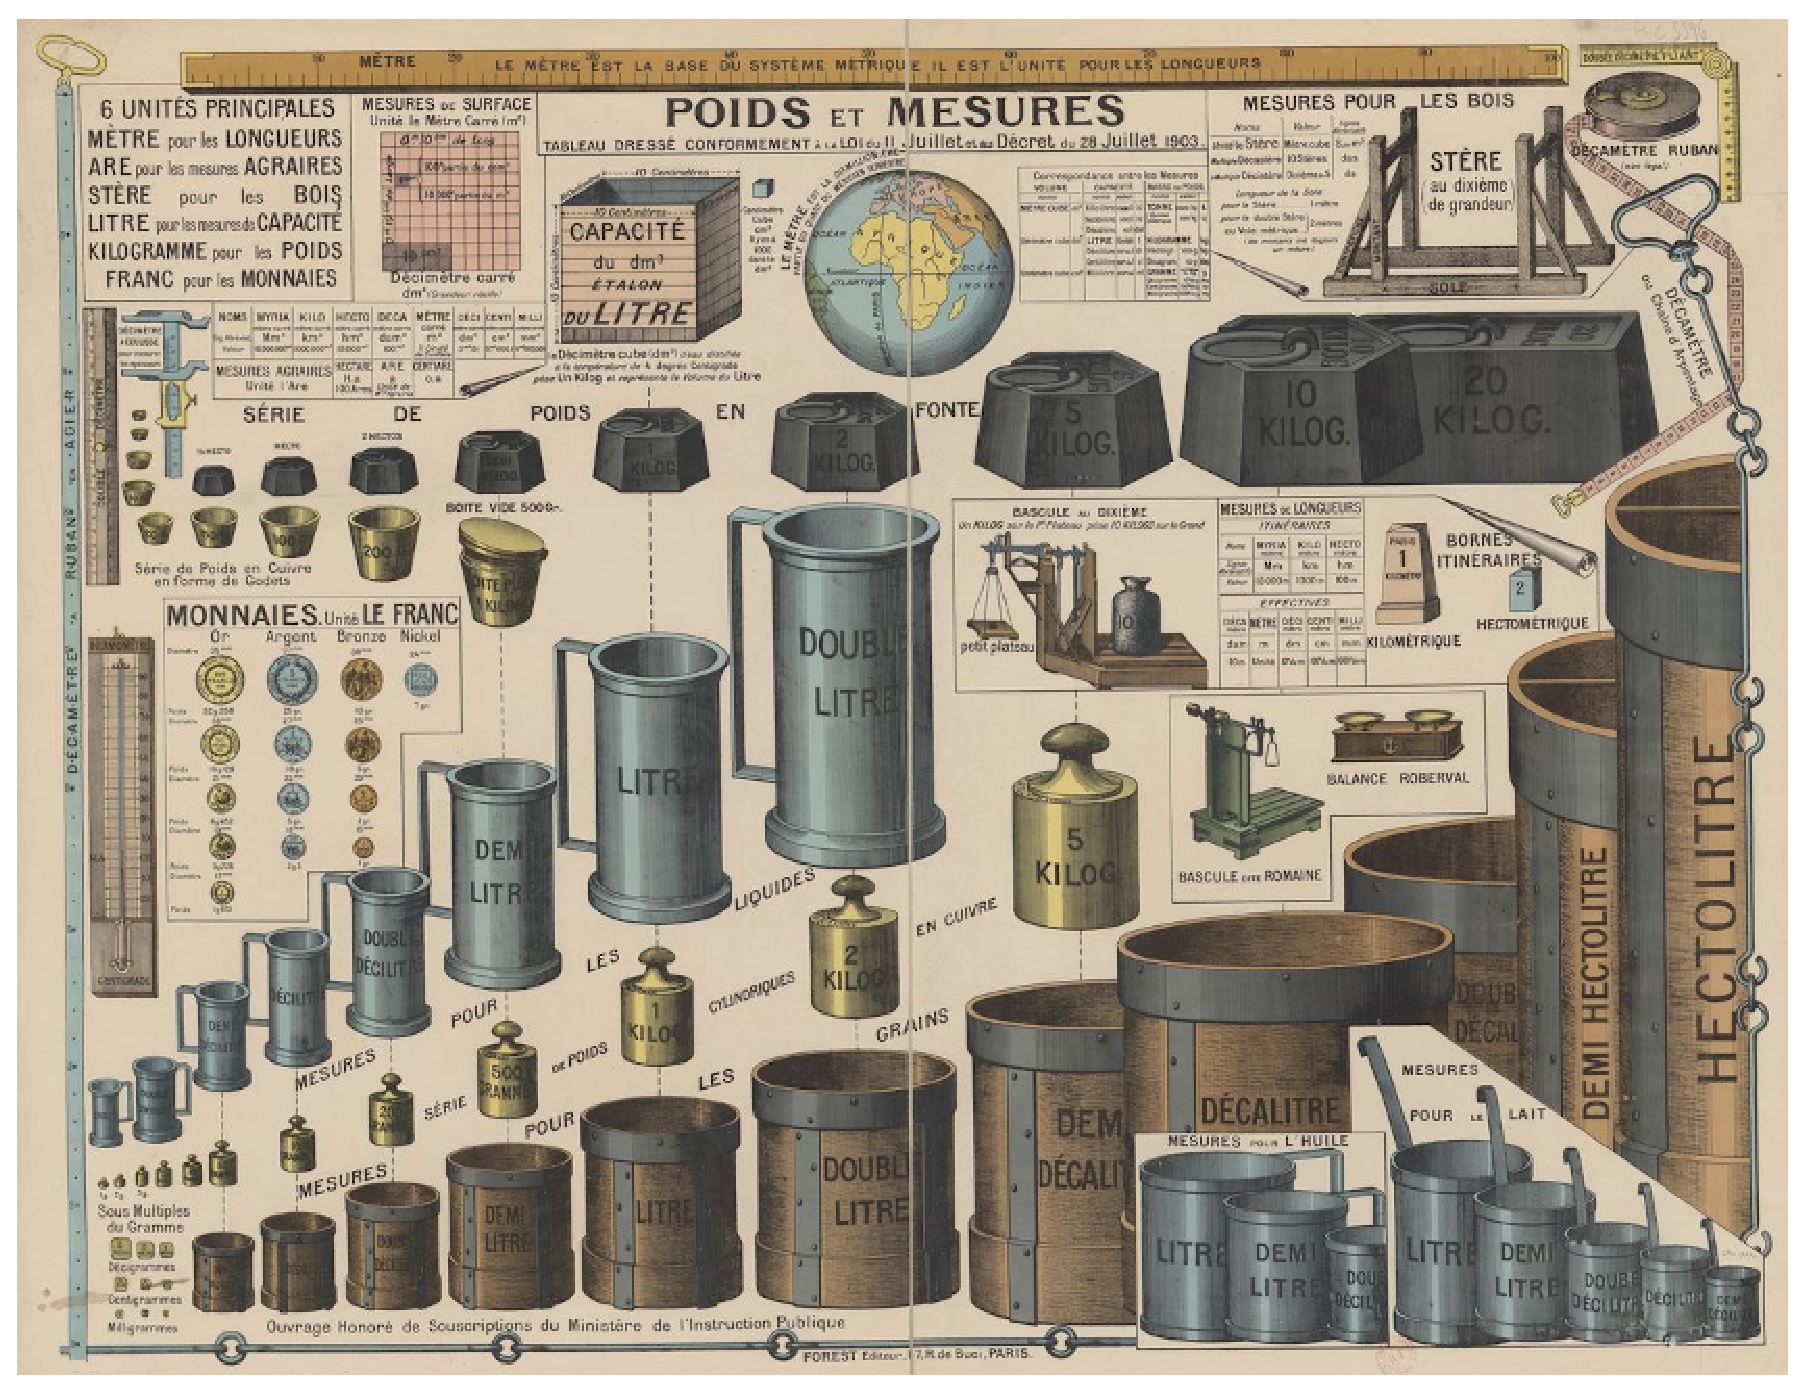
\includegraphics[height=6cm]{Grandeurs_mesures/Images/M13_M14_cours_intro_poids_et_mesures}
   \caption{Poids et mesures. Tableau dressé conformément à la loi du 11 juillet et au décret du 28 juillet 1903}
\end{figure}

\begin{prerequis}[Un peu d'histoire]
Comme vu dans le chapitre précédent, la fin du 18\up{e} siècle se voit doté d'un système métrique universel. Puis, devant la multiplicité d’unités existantes dans les différents pays, la conférence générale des poids et mesures demande à son comité dés 1948 de mettre en place une réglementation complète des unités de mesures. Il ouvre alors une enquête officielle sur l’opinion des milieux scientifiques, techniques et pédagogiques mondiaux afin d’établir un système pratique susceptible d’être adopté par tous les pays. L’accord est réalisé en 1960 sous le nom de système international d’unités (abrégé SI dans toutes les langues). \\
Les unités des grandeurs géométriques, cinématiques et mécaniques sont obtenues par combinaison des trois unités : le mètre (longueur), le kilogramme (masse) et la seconde (durée). Ces trois unités sont appelées unités de base pour cette raison. On a dû ajouter le kelvin (température) et la mole (quantité de matière) pour les grandeurs thermodynamiques ; l'ampère (intensité électrique) pour les grandeurs électriques ; et la candela (intensité lumineuse) pour la photométrie. On doit ajouter deux autres unités purement géométriques : le radian (angle plan) et le stéradian (angle solide), elles sont appelées unités SI supplémentaires ; on peut alors en théorie se contenter de ces neuf unités en fonction desquelles on peut exprimer toutes les grandeurs physiques par combinaisons.
   \end{prerequis}

\cours

\section{Volumes et capacités} % 

\begin{definition}[Volume, capacité et contenance]
   Le \textbf{volume} d’un solide est la place que celui-ci occupe dans l’espace. \\
   La {\bf capacité}, ou la {\bf contenance} d’un récipient, c’est ce qu’il peut contenir.
\end{definition}

\medskip

Ces trois objets n'ont pas la même forme mais occupent la même quantité d'espace, ils ont donc le même volume.  
{\psset{unit=0.6}
   \begin{pspicture}(-6,-1)(13,3.8)
      \psframe[linecolor=A1](0,0)(3,2)
      \psline[linecolor=A1](1,0)(1,2)(1.5,2.5)
      \psline[linecolor=A1](2,0)(2,2)(2.5,2.5)
      \psline[linecolor=A1](0,1)(3,1)(3.5,1.5)
      \psline[linecolor=A1](3,0)(3.5,0.5)(3.5,2.5)(0.5,2.5)(0,2)
      \psline[linecolor=A1](3,2)(3.5,2.5)      
      \pspolygon[linecolor=B2](5,0)(9,0)(9,2)(8,2)(8,1)(6,1)(6,2)(5,2)
      \psline[linecolor=B2](5,1)(6,1)(6,0)
      \psline[linecolor=B2](7,0)(7,1)(7.5,1.5)
      \psline[linecolor=B2](9,0)(9.5,0.5)(9.5,2.5)(8.5,2.5)(8,2)
      \psline[linecolor=B2](9,2)(9.5,2.5)
      \psline[linecolor=B2](9.5,1.5)(9,1)(8,1)(8,0)
      \psline[linecolor=B2](5,2)(5.5,2.5)(6.5,2.5)(6.5,1.5)(8,1.5)
      \psline[linecolor=B2](6,2)(6.5,2.5)
      \psline[linecolor=B2](6,1)(6.5,1.5)      
      \pspolygon[linecolor=G1](11,0)(14,0)(14,1)(13,1)(13,2)(12,2)(12,3)(11,3)
      \psline[linecolor=G1](12,0)(12,1)(11,1)
      \psline[linecolor=G1](13,0)(13,1)(12,1)(12,2)(11,2)
      \psline[linecolor=G1](14,0)(14.5,0.5)(14.5,1.5)(13.5,1.5)(13.5,2.5)(12.5,2.5)(12.5,3.5)(11.5,3.5)(11,3)
      \psline[linecolor=G1](14,1)(14.5,1.5)
      \psline[linecolor=G1](13,2)(13.5,2.5)
      \psline[linecolor=G1](12,3)(12.5,3.5)
      \psline[linecolor=G1](13,1)(13.5,1.5)
      \psline[linecolor=G1](12,2)(12.5,2.5)
   \end{pspicture}}

{\psset{unit=0.6}   
Si l'unité de volume est un cube \quad \psline(0,1)(0,0)(1,0)(1,1)(0,1)(0.5,1.5)(1.5,1.5)(1.5,0.5)(1,0) \psline(1,1)(1.5,1.5) \hspace{1cm}, le volume des ces trois solides est de $6$ unités de volume.}

\begin{exemple*1}
   Pour calculer le volume d'un parallélépipède rectangle, il suffit de \og compter \fg{} le nombre d'unités de volume qu'il comporte. Voici par exemple trois façons de dénombrer :
\vspace*{-0.4cm}
\begin{multicols}{3}
   \begin{center}
      \para{\pspolygon[fillstyle=solid,fillcolor=A1,unit=0.5](0,0)(5,0)(5.5,0.5)(5.5,3.5)(0.5,3.5)(0,3)}     
      \ \\
      face de devant : $3\times5 =15$ \\
      nombre de tranches : $6$ \\
      volume total : $6\times15 =90$
   \end{center} 
   \begin{center}
      \para{\pspolygon[fillstyle=solid,fillcolor=B2,unit=0.5](0,2)(5,2)(8,5)(8,6)(3,6)(0,3)} 
      \ \\
      face du dessus : $5\times6 =30$ \\
      nombre de tranches : $3$ \\
      Volume total : $3\times30 =90$
   \end{center}      
   \begin{center}   
   \para{\pspolygon[fillstyle=solid,fillcolor=G1,unit=0.5](4,0)(5,0)(8,3)(8,6)(7,6)(4,3)}   
       \ \\
      face de côté : $3\times6 =18$ \\
      nombre de tranches : $5$ \\
      Volume total : $5\times18 =90$
   \end{center}
\end{multicols}
\vspace*{-7mm}
\end{exemple*1}

\bigskip

Il existe deux unités principales en dimension 3 : \\
-- les unités de volumes en \og cube \fg{} : c'est également une grandeur composée d'un produit de trois longueurs. \\
-- les unités de capacité ou de contenance en \og litre \fg, unité dérivée des unités de volume. \medskip

\begin{definition}[Mètre cube et litre]
   \begin{itemize}
      \item Lorsque l'unité de volume est un cube de \um{1} d'arête, cela représente {\bf \umc{1}}.
      \item Le {\bf litre} (L) est une unité de capacité valant \udmc{1}. On a alors 1 L = \udmc{1}. \\ [-8mm]
   \end{itemize}
\end{definition}

\bigskip

Pour effectuer un changement d'unité de volume, on reprend les même préfixes que pour les changements de longueur, et on impose pour chacun d'eux trois colonnes au tableau.
\begin{center}
   \begin{ltableau}{0.9\linewidth}{21}
      \hline
      \multicolumn{3}{|c|}{km$^3$} & \multicolumn{3}{c|}{hm$^3$} & \multicolumn{3}{c|}{dam$^3$} & \multicolumn{3}{c|}{m$^3$} & \multicolumn{3}{c|}{dm$^3$} & \multicolumn{3}{c|}{cm$^3$} & \multicolumn{3}{c|}{mm$^3$} \\
      \hline
      & & & & & & & & & & & & \cellcolor{yellow}{\!hL} & \cellcolor{yellow}{\!\!daL} & \cellcolor{yellow}{L}& \cellcolor{yellow}{\!dL} & \cellcolor{yellow}{\!cL} & \cellcolor{yellow}{\!mL} & & & \\
      \hline
      & & & & & & & 2 & 1 & 0 & 9 & 2 & 8 & 0 & 1 & 5 & & & & & \\
      \hline
   \end{ltableau}
\end{center}

Ainsi, pour convertir d'une unité à l'autre; on multiplie ou on divise par \numprint{1000}, \numprint{1000000}\dots

\begin{exemple*1}
    \udamc{21,092801\,5} = \umc{21092,8015} = \uhl{210928,015} = \udmc{21092801,5}\dots
\end{exemple*1}

\begin{tabular}{p{6cm}p{6cm}p{3cm}p{1cm}}
   \begin{minipage}{6cm}
      {\bf Parallélépipède rectangle} \\
      Le {\bf cube} de côté $c$ en est un cas particulier avec $L=\ell=h=c$.
   \end{minipage} 
   &
   \begin{minipage}{6cm}
      \begin{center}
      \psset{yunit=0.9}
         \begin{pspicture}(-0.5,-0.5)(5,3)
            \pspolygon[fillstyle=vlines,hatchcolor=lightgray,linecolor=white](0,0)(3,0)(4,1)(1,1)
            \pspolygon(0,0)(3,0)(4,1)(4,3)(1,3)(0,2)
            \psline(0,2)(3,2)(3,0)
            \psline(3,2)(4,3)
            \psline[linestyle=dashed](0,0)(1,1)(4,1)
            \psline[linestyle=dashed](1,1)(1,3)
            \psset{linecolor=B1}
            \psline{<->}(0,-0.3)(3,-0.3)
            \rput(1.5,-0.6){\textcolor{B1}{$L$}}
            \psline{<->}(-0.3,0)(-0.3,2)
            \rput(-0.6,1){\textcolor{B1}{$\ell$}}
            \psline{<->}(-0.2,2.2)(0.9,3.3)
            \rput(0.2,3){\textcolor{B1}{$h$}}
         \end{pspicture}
      \end{center}
   \end{minipage}
   &
   \begin{minipage}{4cm}
      ${\cal V}=L\times \ell\times h$ \\
      cube : ${\cal V}=c^3$
   \end{minipage}
   &
   \multirow{8}{*}{\rotatebox{-90}{\hspace*{1.6cm} Aire de la base $\times$ hauteur}} \\
   & & & \\
   & & & \\
   \begin{minipage}{6cm}
      {\bf Prisme} \\
      $\cal A$ est l'aire d'une base, $h$ la hauteur du prisme.
   \end{minipage}
   &
   \begin{minipage}{6cm}
      \begin{center}
         \begin{pspicture}(-0.75,0)(5,3)
            \pspolygon[fillstyle=vlines,hatchcolor=lightgray,linecolor=white](0,0.5)(1,0)(3.5,1)(2.5,1.5)(1.5,1.5)
            \psline(0,2)(1.5,3)(2.5,3)(3.5,2.5)(1,1.5)(0,2)(0,0.5)(1,0)(3.5,1)(3.5,2.5)
            \psline(1,0)(1,1.5)
            \psline[linestyle=dashed](0,0.5)(1.5,1.5)(2.5,1.5)(3.5,1)
            \psline[linestyle=dashed](1.5,1.5)(1.5,3)
            \psline[linestyle=dashed](2.5,1.5)(2.5,3)
            \psline[linecolor=B1]{<->}(-0.25,0.5)(-0.25,2)
            \rput(-0.55,1.25){\textcolor{B1}{$h$}}
            \rput(1.75,0.9){\textcolor{B1}{$\mathcal{A}$}}
         \end{pspicture}
      \end{center}
   \end{minipage}
   &
   ${\cal V}={\cal A}\times h$
   & \\
   & & & \\
   \begin{minipage}{6cm}
      {\bf Cylindre} \\
      $h$ est la hauteur du cylindre, et $r$ est le rayon du disque de base.
   \end{minipage}
   &
   \begin{minipage}{6cm}
      \begin{center}
         \begin{pspicture}(-0.5,0.5)(5,3.5)
            \psline(0.5,1)(3.5,1)
            \psline(0.5,3)(3.5,3) 
            \psellipse(3.5,2)(0.3,1) 
            \psellipse[fillstyle=vlines,hatchcolor=lightgray,linecolor=white](0.5,2)(0.3,1)
            \psellipticarc[linestyle=dashed](0.5,2)(0.3,1){-90}{90}
            \psellipticarc(0.5,2)(0.3,1){90}{-90}
            \psset{linecolor=B1}
            \psline{<->}(0.5,2)(3.5,2)
            \rput(2,2.3){\textcolor{B1}{$h$}}
            \psline{<->}(0.5,1)(0.5,2)
            \rput(0.35,1.6){\textcolor{B1}{$r$}}
         \end{pspicture}
      \end{center}
   \end{minipage}
   &
   ${\cal V}=\pi\,r^2\, h$
   & \\
   & & & \multirow{6}{*}{\rotatebox{-90}{\hspace*{1.3cm}  Aire de la base $\times$ hauteur $\div$ 3}} \\
   \hline
   & & & \\
   \begin{minipage}{6cm}
   {\bf Cône} \\
      $r$ est le rayon du disque de base et $h$ la hauteur du cône.
   \end{minipage}
   &
   \begin{minipage}{6cm}
      \begin{center}
         \begin{pspicture}(-0.5,0.3)(5,3.5)
            \psline(0.5,1)(3.5,2)(0.5,3)
            \psellipse[fillstyle=vlines,hatchcolor=lightgray,linecolor=white](0.5,2)(0.3,1)
            \psellipticarc[linestyle=dashed](0.5,2)(0.3,1){-90}{90}
            \psellipticarc(0.5,2)(0.3,1){90}{-90}
            \psset{linecolor=B1}
            \psline{<->}(0.5,2)(3.5,2)
            \rput(1.8,2.3){\textcolor{B1}{$h$}}
            \psline{<->}(0.5,1)(0.5,2)
            \rput(0.35,1.6){\textcolor{B1}{$r$}}
         \end{pspicture}
      \end{center}
   \end{minipage}
   &
   ${\cal V}=\dfrac{1}{3}\times\pi\,r^2\,h$
   & \\
   \begin{minipage}{6cm}
      {\bf Pyramide} \\
      $\cal A$ est l'aire de la base et $h$ la hauteur de la pyramide.
   \end{minipage}
   &
   \begin{minipage}{6cm}
      \begin{center}
         \begin{pspicture}(-0.75,0)(5,3.5)
            \pspolygon[fillstyle=vlines,hatchcolor=lightgray,linestyle=dashed](0,0.5)(1,0)(3.5,1)(2.6,1.4)(1.6,1.5)
            \pspolygon(2,3.5)(0,0.5)(1,0)(3.5,1)
            \psline(1,0)(2,3.5)
            \psline[linestyle=dashed](2.6,1.4)(2,3.5)
            \psline[linestyle=dashed](1.6,1.5)(2,3.5)
            \psline[linecolor=B1]{<->}(2,3.5)(2,1)
            \rput(2.2,2){\textcolor{B1}{$h$}}
            \rput(1.7,0.9){\textcolor{B1}{$\mathcal{A}$}}
         \end{pspicture} \newline
      \end{center}
   \end{minipage}
   &
   ${\cal V}=\dfrac{1}{3}\times{\cal A}\,h$
   & \\
   \hline
   & & & \\
   \begin{minipage}{6cm}
      {\bf Sphère} ou {\bf Boule} \\
      $r$ est le rayon.  
   \end{minipage}
   &
   \begin{minipage}{6cm}
      \begin{center}
         \begin{pspicture}(-0.5,0.5)(5,3.5)
            \pscircle(2,2){1.5}
            \psellipticarc[linestyle=dashed](2,2)(1.5,0.5){0}{180}
            \psellipticarc(2,2)(1.5,0.5){180}{0}
            \psline[linecolor=B1]{<->}(2,2)(3.5,2)
            \rput(2.75,2.2){\textcolor{B1}{$r$}}
         \end{pspicture}
      \end{center}
   \end{minipage}
   &
   ${\cal V}=\dfrac{4}{3}\times\pi\,r^3$
   & \\
\end{tabular}


%%%%%%%%%%%%%%%%%
\section{Durées et horaires} % 
    
La seconde (s) est l'unité du système SI permettant de caractériser une durée. Contrairement aux autres unités, elle ne suit pas un système décimal, mais hexadécimal (de base 60).

\begin{pspicture}(-3,0)(5,3.3)
   \rnode{A}{\psframebox{durée en heures}}
   \hspace{12mm}
   \rnode{B}{\psframebox{durée en minutes}}
   \hspace{12mm}
   \rnode{C}{\psframebox{durée en secondes}}
   \nccurve[angle=90,linecolor=A1,offset=-1mm]{A}{B}
   \naput*{\textcolor{A1}{$\stackrel{\times60}{\longrightarrow}$}}
   \nbput*{\textcolor{A1}{$\stackrel{\div60}{\longleftarrow}$}}
   \nccurve[angle=90,linecolor=A1,offset=-1mm]{->}{B}{C}
   \naput*{\textcolor{A1}{$\stackrel{\times60}{\longrightarrow}$}}
   \nbput*{\textcolor{A1}{$\stackrel{\div60}{\longleftarrow}$}}
   \nccurve[angle=90,linecolor=B1]{->}{A}{C}
   \naput*{\textcolor{B1}{$\stackrel{\times3\,600}{\longrightarrow}$}}
   \nbput*{\textcolor{B1}{$\stackrel{\div3\,600}{\longleftarrow}$}}
\end{pspicture}

\begin{exemple}
\ \\ [-10mm]
   \begin{itemize}
      \item Convertir $170$ minutes en heures et minutes.     
      \item Convertir $1$ h $25$ min $36$ s en secondes.
   \end{itemize}
\correction
\ \\ [-10mm]
\begin{itemize}
      \item $170=2\times60+50$, donc 170 min = 2 h 50 min.
      \item 1 h = 3\,600 s et 1 min = 60 s donc \\
      1 h 25 min 36 s = 3\,600\ s + $25\times60$ s + 36 s = 5\,136 s.
   \end{itemize}
\end{exemple}

\bigskip

Pour effectuer des additions ou soustractions de durées, on peut effectuer une opération en colonne (un peu périlleuse) ou procéder de proche en proche.
 
\begin{exemple}
\ \\ [-10mm]
  \begin{itemize}
      \item Un train part de Montpellier à \\
      8 h 48 min. La durée du trajet pour se rendre à Paris est de 3 h et 20 min. \\
      À quelle heure arrivera-t-il à Paris ?
      \item Un automobiliste part de Perpignan à 8 h 35 min et arrive à Montpellier à 10~h~20~min. Quelle est la durée de son trajet ?
   \end{itemize}
\correction
\ \\ [-8mm]
   \begin{itemize}
      \item   
      \begin{tabular}{ccccc}
         & 8 & h & 4 & 8 \\
         $+$ & 3 & h & 2 & 0 \\
         \hline
         1 & $\cancel{1}$ & h & $\cancel{6}$ & 8 \\
         \multicolumn{5}{c}{\psline{->}(0.5,0.3)(-0.5,-0.1)} \\
         1 & 2 & h & 0 & 8
      \end{tabular}
      \quad
      \begin{tabular}{p{5cm}}
        {\small on aligne les heures sous les heures, les minutes sous les minutes puis on additionne terme à terme. Si le nombre de minutes est supérieur à 60, on soustrait 60 min et on ajoute 1 h.} \\
      \end{tabular} 
      \medskip
      \item 8 h 35 $\xrightarrow{+\text{25 min}}$ 9 h 00 $\xrightarrow{+\text{1 h}}$ 10 h 00 $\xrightarrow{+\text{20 min}}$ 10 h 20. \\   
      La durée totale du trajet est de 1 h 45 min.
   \end{itemize}   
\end{exemple}

\begin{remarque}
   attention à l'aspect hexadécimal de cette grandeur :
   \begin{itemize}
      \item lorsqu'on lit 1,5 h, cela correspond à 1 h et 0,5 h, c'est-à-dire 1h et 30 min ($0,5\times 60$ min).
      \item Inversement, 2 h 15 min ne correspond pas à 2,15 h mais à 2,25 h (15 min = $\dfrac{15}{60}$ h = 0,25 h).
   \end{itemize}
\end{remarque}


%%%%%%%%%%%%%%%%%%%
\section{Masse}

   On peut mesurer une masse grâce au gramme (g) et à toutes les unités qui en découlent. Pour désigner les multiples ou les subdivisions des mesures, on utilise les préfixes identiques à ceux déjà utilisés pour les unités de longueurs :
   \begin{center}
   \renewcommand{\arraystretch}{1.2}
   \begin{CLtableau}{0.8\linewidth}{8}{p{3cm}}
      \hline
      Préfixe & kilo & hecto & déca & & déci & centi & milli \\
      \hline
      Signification & 1\,000 & 100 & 10 & 1 & $\dfrac{1}{10}$ &
      $\dfrac{1}{100}$ & $\dfrac{1}{1\,000}$ \\ [3mm]
      \hline
      Unité de masse & kg & hg & dag & g & dg & cg & mg \\
      \hline
   \end{CLtableau}
   \end{center}

\begin{remarque}
   on utilise aussi la tonne pour les masses plus importantes selon la correspondance suivante : 1 tonne = 1\,000 kg.
\end{remarque}



%%%%%%%%%%%%%%%%%
\section{Grandeurs composées} % 

\begin{definition}[Grandeur composée]
   Une {\bf grandeur composée} est une grandeur qui s'exprime en fonction de plusieurs unités de base : grandeur produit lorsqu'on les multiplie et grandeur quotient lorsqu'on les divise.
\end{definition}

\bigskip

Pour les grandeurs composées, il est essentiel de faire attention à la cohérence des unités. \\
Quelques exemples, bien évidement non exhaustifs ;-)
\begin{center}
   \begin{tabular}{|C{1}|C{8}|C{5}|}
      \hline
      \multirow{2}{*}{\rotatebox{90}{Grandeurs produit}}
      &
      \begin{pspicture}(0,0.9)(8,3.5)
         \rput(4,2.3){L'aire est le produit}
         \rput(4,1.8){de deux longueurs.}
      \end{pspicture}
      &
      \begin{pspicture}(0,0.9)(4,3.5)
         \rput(2,1.5){\large $\mathcal{A}_{\text{triangle}} =\dfrac{b\times h}{2}$}
         \psline[linecolor=gray]{->}(2.6,2.1)(2.6,2.7)
         \rput(3,3){\blue cm $\times$ cm}
         \psline[linecolor=gray]{->}(3.3,2.1)(3.3,2.7)
         \rput(1.1,3.05){\blue cm$^2$}
         \psline[linecolor=blue]{->}(2.1,3)(1.6,3)
         \psline[linecolor=gray]{->}(1.1,2.7)(1.1,1.7)
      \end{pspicture}
      \\
      \cline{2-3}
      &
      \begin{pspicture}(0,1)(8,3.4)
         \rput(4,2.4){Le poids est le produit d'une masse par}
         \rput(4,1.9){l'intensité de la pesanteur (9,81 N/kg à Paris).}
      \end{pspicture}
      &
      \begin{pspicture}(0,1)(4,3.4)
         \rput(2,1.5){\large $\mathcal{P} =m\times g$}
         \psline[linecolor=gray]{->}(2.1,1.8)(2.1,2.4)
         \rput(2.7,2.7){\blue kg $\times$ N/kg}
         \psline[linecolor=gray]{->}(2.9,1.8)(2.9,2.4)
         \rput(1.2,2.7){\blue N}
         \psline[linecolor=blue]{->}(1.8,2.7)(1.4,2.7)
         \psline[linecolor=gray]{->}(1.2,2.4)(1.2,1.8)
      \end{pspicture}
      \\
      \hline
      \multirow{2}{*}{\rotatebox{90}{Grandeurs quotient}}
      &
      \begin{pspicture}(0,-0.1)(8,3.5)
         \rput(4,1.8){La vitesse est le quotient}
         \rput(4,1.3){d'une distance par un temps.}
      \end{pspicture}
      &
      \begin{pspicture}(-1,-0.1)(3,3.5)
         \rput(2,1.5){\large $v =\dfrac{d}{t}$}
         \psline[linecolor=gray]{->}(2.4,2.1)(2.4,2.6)
         \rput(2.4,2.9){\blue m}
         \psline[linecolor=gray]{->}(2.4,0.9)(2.4,0.4)
         \rput(2.4,0.2){\blue s}
         \rput(0.2,1.5){\blue m/s}
         \psline[linecolor=blue]{->}(2.1,2.8)(0.2,1.8)
         \psline[linecolor=blue]{->}(2.1,0.3)(0.5,1.2)
         \psline[linecolor=gray]{<-}(0.7,1.45)(1.3,1.45)
      \end{pspicture}
      \\
      \cline{2-3}
      &
      \begin{pspicture}(0,-0.1)(8,3.5)
         \rput(4,1.8){La masse volumique est le quotient}
         \rput(4,1.3){d'une masse par un volume.}
      \end{pspicture}
      &
      \begin{pspicture}(-1,-0.1)(3,3.5)
         \rput(2,1.5){\large $\rho =\dfrac{m}{V}$}
         \psline[linecolor=gray]{->}(2.4,2.1)(2.4,2.6)
         \rput(2.4,2.9){\blue g}
         \psline[linecolor=gray]{->}(2.4,0.9)(2.4,0.4)
         \rput(2.4,0.2){\blue cm$^3$}
         \rput(0.2,1.5){\blue g/cm$^3$}
         \psline[linecolor=blue]{->}(2.1,2.8)(-0.1,1.8)
         \psline[linecolor=blue]{->}(2.1,0.3)(0.4,1.2)
         \psline[linecolor=gray]{<-}(0.7,1.45)(1.3,1.45)
      \end{pspicture}
      \\
      \hline
   \end{tabular}
\end{center}

\bigskip

Moyen mnémotechnique pour passer d'une écriture à l'autre dans une grandeur quotient : \\
on considère, par exemple, l'expression de la vitesse que l'on peut modéliser de la manière suivante :
\begin{center}
   \begin{pspicture}(-2.2,0)(5,3.8)
      \pspolygon[fillstyle=solid,fillcolor=yellow!50](0,0)(3,0)(1.5,2.6)
      \psline[linecolor=blue,linewidth=0.5mm](0.7,1.2)(2.3,1.2)
      \psline(1.5,0)(1.5,1.2)
      \rput(1,0.6){\Large $v$}
      \rput(2,0.6){\Large $t$}
      \rput(1.5,1.7){\Large $d$}
      \rput(1.5,0.6){\red\Large $\times$}
      \rput(-1.5,0.6){\Large $v =\Dfrac{d}{t}$}
      \rput(1.5,3.2){\Large $d =v{\red \times}t$}
      \rput(4.3,0.6){\Large $t =\Dfrac{d}{v}$}
   \end{pspicture}
\end{center}


%%%%%%%%%%%%%%%%%%%%%%%%%%%%%%%
%%%%%%%%%%%%%%%%%%%%%%%%%%%%%%%
\activites

%%%
\begin{activite}[Groupement 1 - Exercice 5 - Question 1 : Volume et capacité]
   \ \\ [-16mm]
   \begin{QCM}
      \begin{minipage}{12cm}
         Un ballon-sonde est un ballon à gaz utilisé pour faire des mesures locales dans l'atmosphère. \\
         Dans le cadre du projet scientifique qu’elle anime pour sa classe de CM2, une professeure des écoles a reçu un petit ballon-sonde, représenté ci-contre. \\  
         Son enveloppe, composée de matières plastiques et de latex, a la forme, une fois gonflée, d'un cône de révolution surmonté d'une demi-sphère. \\ 
         Les dimensions données sur la figure ci-contre sont celles du ballon-sonde au sol, sur le lieu du lâcher situé au niveau de la mer.
      \end{minipage}
      \qquad
      \begin{minipage}{6cm}
         {\psset{unit=0.5}
         \footnotesize
         \begin{pspicture}(0,1)(5,7.8)
            \psline(5,5.9)(3,0)(1,5.9)
            \psellipticarc(3,6)(2,0.7){180}{0}
            \psellipticarc[linestyle=dotted](3,6)(2,0.7){0}{180}
            \psarc(3,6){2}{0}{180}
            \psline[linestyle=dashed](3,0)(3,6)(5,6)
            \psframe(3,6)(3.2,5.8)
            \rput{-90}(3.5,3.1){90 cm}
            \rput(4,6.3){30 cm}
            \psarc(3,0){1.2}{70}{90}
            \rput(3.25,1.5){$\alpha$}
            \rput(3,-0.3){$S$}
            \rput(2.7,6.3){$O$}
            \rput(5.3,6){$N$}      
         \end{pspicture}}
      \end{minipage} \\ [2mm]
     {\it On pourra, si nécessaire, utiliser le formulaire ci-dessous.}
     \begin{center}
         {\small
         \begin{tabular}{|C{4}|C{5.5}|C{4}|}
            \hline
            \begin{pspicture}(-2,-1.5)(2,1.5)
               \footnotesize\pscircle(0,0){1}
               \psline[linestyle=dashed](0,0)(1,0)
               \rput(-0.2,0){$O$}
               \rput(0.5,0.2){$r$}
            \end{pspicture}
            &
            {\psset{unit=0.5}
            \footnotesize
            \begin{pspicture}(1,0)(10,6.5)
               \psline(5,1)(3,6)(1,1)
               \psellipticarc(3,1)(2,0.8){180}{0}
               \psellipticarc[linestyle=dotted](3,1)(2,0.8){0}{180}
               \psline[linestyle=dashed](5,1)(3,1)(3,6)
               \rput(3.3,3){$h$}
               \rput(4,1.2){$r$}
               \rput(4.3,3.5){$g$}
               \rput(2.7,1){$O$}
               \rput(3,6.4){$S$}
               \rput(8,5){\parbox{2.8cm}{$g$ est la longueur d'une génératrice du cône}}
            \end{pspicture}}
            &
            \begin{pspicture}(-2,-1.5)(2,1.5)
               \footnotesize\pscircle(0,0){1}
               \psellipticarc(0,0)(1,0.6){180}{0}
               \psellipticarc[linestyle=dotted](0,0)(1,0.6){0}{180}
               \psline[linestyle=dashed](0,0)(1,0)
               \rput(-0.2,0){$O$}
               \rput(0.5,0.2){$r$}
            \end{pspicture} \\
            \hline
            Périmètre du disque : $2\,\pi\,r$& Volume du cône : $\dfrac13\,\pi\,r^2\,h$& Volume de la boule :$\dfrac43\,\pi\,r^3$ \\
            \hline
            Aire du disque : $\pi\,r^2$ & Aire de la surface latérale : $\pi\,r\,g$ & Aire de la sphère : $4\,\pi\,r^2$ \\
            \hline
         \end{tabular}}
      \end{center}
      \begin{enumerate}
         \item Montrer, en indiquant les étapes du calcul, que le volume exact du ballon-sonde au niveau de la mer, est égal à 45 000 $\pi$ cm$^3$.   
         \item Donner le volume du ballon sonde en litre, arrondi à l’entier. \\ [-8mm]
      \end{enumerate}
   \end{QCM}
   
   \bigskip
   
   \textcolor{G1}{
   {\bf Exemple de corrigé.} \smallskip
   \begin{enumerate}
      \item Calcul du volume de la partie conique : $V_1 =\dfrac13\times\pi\times(30\text{ cm})^2\times90\text{ cm} =27\,000\,\pi\text{ cm}^3$. \\ [1mm]
         Calcul du volume de la demi-sphère : $V_2 =\dfrac12\times\left(\dfrac43\times\pi\times(30\text{ cm})^3\right)=18\,000\,\pi\text{ cm}^3$. \\ [1mm]
         Calcul du volume du ballon-sonde : $V =V_1+V_2  =27\,000\,\pi\text{ cm}^3+18\,000\,\pi\text{ cm}^3 =45\,000\,\pi\text{ cm}^3$. \\ [1mm]
         \uline{Le volume du ballon-sonde au niveau de la mer est de $45\,000\,\pi\text{ cm}^3$}
      \item Grâce a la correspondance \og $1\text{dm}^3 =1\text{ L}$ \fg, on a : $V =45\,000\,\pi\text{ cm}^3 =45\,\pi\text{ dm}^3 =45\,\pi\text{ L} \approx141,37$. \\
         \uline{Le ballon a un volume d'environ 141 litres}. \medskip
   \end{enumerate}}
\end{activite}

\bigskip


%%%
\begin{activite}[Groupement 3 - Exercice 1 - Question 1 : Volume]
   \ \\ [-16mm]
   \begin{QCM}
      \begin{center}
         \begin{tabular}{|p{8cm}|*{4}{C{1.3}|}}
            \hline
            \bf Question : & \bf A & \bf B & \bf C & \bf D \\
            \hline
            Quel est le volume d’un cylindre d’une hauteur de \ucm{6} et de base un disque d’un diamètre de \ucm{8} ?
            & $48\,\pi\,\ucmq{}$
            & $96\,\pi\,\ucmq{}$
            & $144\,\pi\,\ucmq{}$
            & $384\,\pi\,\ucmq{}$ \\
            \hline
         \end{tabular} \medskip
      \end{center}
   \end{QCM}
   
   \bigskip
   
   \textcolor{G1}{
   {\bf Exemple de corrigé.} \\ \smallskip
      $\mathcal{V} =\pi\times r^2\times h =\pi\times(\ucm{4})^2\times\ucm{6} =96\,\pi\,\ucmq{}$. \uline{La bonne réponse est B}.}
\end{activite}

\pagebreak


%%%%%%%%%%%%%%%%%%%%%%%%%%%%%%%
%%%%%%%%%%%%%%%%%%%%%%%%%%%%%%%
\begin{activite}[Groupement 3 - Exercice 3 - Partie B : Volume, capacité et prix]
   \ \\ [-16mm]
   \begin{QCM}
      Dans cette partie, un jardin est assimilé à un rectangle qui a pour longueur \um{12} et pour largeur \um{5}. \\
      On souhaite entourer le jardin d’une bordure de \ucm{30} de hauteur afin de remplir le pavé droit obtenu d’un mélange de terre et de terreau. On négligera, dans cette partie, l’épaisseur de la bordure du jardin. \\
Le mélange est composé d’un tiers de terreau et de deux tiers de terre.
\begin{center}
   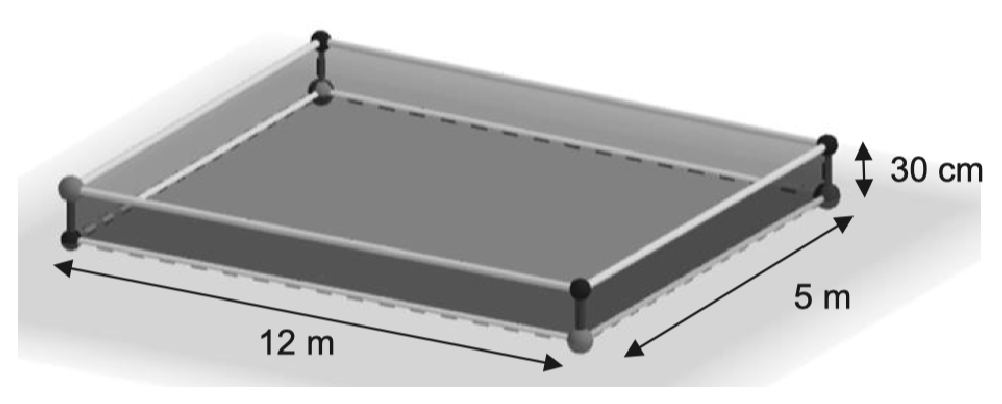
\includegraphics[width=6cm]{Grandeurs_mesures/Images/M14_ex_jardin}
\end{center}
\begin{enumerate}
   \item Montrer que le volume de terreau nécessaire pour le potager est de 6 m$^3$.
   \item Trois magasins proposent les offres suivantes : \\ [2mm]
      \fbox{
         \begin{minipage}{4cm}
            \centering{\bf Magasin 1} 
            \flushleft Livraison : 20 \euro \\
            0,10 \euro{} le litre de terreau
         \end{minipage}}
      \quad
      \fbox{
         \begin{minipage}{6cm}
            \centering{\bf Magasin 2}
            \flushleft Livraison offerte \\
            2,35 \euro{} le sac de 20 litres de terreau \\
            20\,\% de remise immédiate après l’achat d’une carte de fidélité au prix de 10 \euro
         \end{minipage}} 
      \quad
      \fbox{
         \begin{minipage}{4cm}
            \centering{\bf Magasin 3}
            \flushleft Livraison offerte pour tout achat supérieur à 50 \euro \\
            5,37 \euro{} le sac de 50 litres de terreau 
         \end{minipage}} \\ [2mm]
      Quel magasin choisir pour avoir le tarif, livraison comprise, le plus économique pour les \umc{6} nécessaires ? \\ [-8mm]
\end{enumerate}

   \end{QCM}
   
   \bigskip
   
   \textcolor{G1}{
   {\bf Exemple de corrigé.} \smallskip
      \begin{enumerate}
         \item On commence par calculer le volume du bac  : \\
      $\mathcal{V} =\text{longueur}\times\text{largeur}\times\text{hauteur} =\um{12}\times\um{5}\times\um{0,3} =\umc{18}$. \\ [0.5mm]
            Le remplissage nécessite un tiers de terreau, soit $\dfrac13\times\umc{18} =\umc{6}$. \\ [0.5mm]
            \uline{On a besoin de \umc{6} de terreau pour remplir le potager}.
         \item On calcule le coût pour \umc{6} pour chaque magasin, sachant que 6 m$^3$ = 6 000 dm$^3$ = 6 000 L.  
            \begin{itemize}
               \item Magasin 1. \\ [1mm]
                  $\Imp{\text{Prix du terreau : } 6\,000\times0,10\text{ \euro}=600\text{ \euro}}{\text{Prix de la livraison : }20\text{ \euro}}$ Prix total : 600 \euro{} + 20 \euro{} = 620 \euro.
                  \item Magasin 2 sans carte de fidélité. \\
                  $\Imp{\text{Prix du terreau : } \dfrac{6\,000}{20}\times2,35\text{ \euro}=705\text{ \euro}}{\text{Prix de la livraison : offerte}}$ Prix total : 705 \euro. \\ [1mm]
                  Magasin 2 avec carte de fidélité. \\
                  $\Impl{\text{Prix du terreau : } \left(1-\dfrac{20}{100}\right)\times\dfrac{6\,000}{20}\times2,35\text{ \euro}=564\text{ \euro}}{\text{Prix de la livraison : offerte}}{\text{Prix de la carte de fidélité : 10 \euro}}$ Prix total : 564\text{ \euro} + 10\text{ \euro} = 574\text{ \euro}.
                 \item Magasin 3. \\
                  $\Imp{\text{Prix du terreau : } \dfrac{6\,000}{50}\times5,37\text{ \euro}=644,40\text{ \euro}}{\text{Prix de la livraison : offerte}}$ Prix total : 644,40 \euro. \\ [1mm]
                  \uline{Le magasin le plus économique est le magasin 2, en prenant la carte de fidélité}.
               \end{itemize}
      \end{enumerate}}
\end{activite}

\pagebreak


%%%
\begin{activite}[Groupement 2 - Exercice 3 - Partie 1 - Question 3 : Volumes]
   \ \\ [-16mm]
   \begin{QCM}
      \begin{minipage}{9cm}
         On considère un pavé droit $ABCDA’B’C’D’$ avec \\
         $DD’ =\ucm{5}$ ; $DC =\ucm{6}$ et $DA =\ucm{7}$. \\
         On note $L$ le point d’intersection des diagonales $[AC]$ et $[BD]$. \\
         On souhaite creuser ce pavé, en retirant une pyramide $OABCD$ de hauteur $[OL]$. \\
         Dans cette partie, on suppose que $OL =4$ cm.
         \begin{enumerate}
            \item Calculer le volume de la pyramide $OABCD$.           
            \item Calculer le volume du pavé creusé.
         \end{enumerate}
      \end{minipage}
      \begin{minipage}{7cm}
         \begin{pspicture}(-1,-1)(6,4.2)
         \psset{yunit=1.4}
            \pstGeonode[CurveType=polygon,PointSymbol=none,PosAngle={-135,-45,0,45,135,135},PointName={D',C',B',B,A,D}](0,0){D'}(4,0){C'}(5.5,0.7){B'}(5.5,2.7){R}(1.5,2.7){S}(0,2){D}
            \small
            \pstGeonode[PointSymbol=none,PosAngle={90,-90,135,90}](4,2){C}(2.75,1){O}(1.5,0.7){A'}(2.75,2.35){L}
            \pstLineAB{D}{C}
            \pstLineAB{C}{R}
            \pstLineAB{C}{C'}
            \psset{linestyle=dashed}
            \pstLineAB{D'}{A'}
            \pstLineAB{A'}{B'}
            \pstLineAB{S}{A'}
            \psset{linestyle=dotted}
            \pstLineAB{D}{R}
            \pstLineAB{S}{C}
            \pstLineAB{S}{O}
            \pstLineAB{R}{O}
            \pstLineAB{C}{O}
            \pstLineAB{D}{O}
            \pstLineAB{L}{O}
         \end{pspicture}
      \end{minipage} 
   \end{QCM}
   
   \bigskip
   
   \textcolor{G1}{
   {\bf Exemple de corrigé.} \smallskip
      \begin{enumerate}
         \item $\mathcal{V} =\dfrac13\times\mathcal{A}_{ABCD}\times OL =\dfrac13\times6\text{ cm}\times7\text{ cm}\times4\text{ cm} =56\text{ cm}^3$. \\ [1mm]
            \uline{Le volume de la pyramide est égal à 56 cm$^3$}.
         \item Le volume du pavé creusé s'obtient en soustrayant le volume de la pyramide $OABCD$ au volume du pavé droit $ABCDA'B'C'D'$ : \\
            $\mathcal{V} =5\text{ cm}\times6\text{ cm}\times7\text{ cm}-56\text{ cm}^3 =210\text{ cm}^3-56\text{ cm}^3 =154\text{ cm}^3$. \\ [1mm]
            \uline{Le volume du pavé creusé est égal à 154 cm$^3$}.
      \end{enumerate}}
\end{activite}


%%%%%%%%%%%%%%%%%%%%%%%%%%%%%%
%%%%%%%%%%%%%%%%%%%%%%%%%%%%%%
\exercicesbase

\begin{center}
   {\cursive Maîtriser les bases avec} \href{http://mathenpoche.sesamath.net}{
\includegraphics[width=3cm]{Nombres_et_calculs/Images/mathenpoche}} \\
   \bigskip
   {\hautab{0.85}
   \cursive
   \begin{Ltableau}{0.775\linewidth}{4}{C{1}|C{1}|p{7cm}|p{2.3cm}}
      \hline
      Classe & \texttt{N\degre} & Thème & Dans le cours \\
      \hline
      \textcolor{orange}{\bf 6\up{e}} & \texttt{G1} & Durées & 2. \\
      \hline
       & \texttt{G6} & Volumes & 1. \\
      \hline
      \textcolor{cyan}{\bf 5\up{e}} & \texttt{C} & Grandeurs et mesures & 1. et 3. \\
      \hline
      \textcolor{violet}{\bf 4\up{e}} & \texttt{G2} & Calculs de volume & 1. \\
      & \texttt{G4} & Grandeurs composées & 3. \\
      \hline
      \textcolor{teal}{\bf 3\up{e}} & \texttt{G1} & Calculs de volume & 1. \\
      & \texttt{G2} & Grandeurs composées & 3. \\
      \hline
\end{Ltableau}}
\end{center}

\bigskip


\begin{exercice}[CRPE 2005 Lyon] %%%1
   On rappelle que la masse volumique d'un corps, solide ou liquide, est le quotient de sa masse par son volume ; la masse volumique de l'eau est, dans des conditions normales, 1 g/\ucmc{}. \\
   Une statuette métallique a une masse de \ug{340}. On dispose d'un vase, dont la masse (à vide !) est \ug{500}. On remplit à ras bord le vase d'eau, l'ensemble pèse \ug{2300}. \\
   Si on immerge la statue dans le vase plein, on trouve après débordement que le vase pèse \ug{2600}.
   \begin{enumerate}
      \item Calculer le volume de la statue.
      \item Calculer la masse volumique de la statue en g/\ucmc{}, puis en kg/L (kilogramme par litre).
      \item On vide le vase de l'eau et de la statue, puis on le remplit à ras bord d'un nouveau liquide. L'ensemble pèse \ug{1940}. Quelle est la masse volumique de ce liquide ?
   \end{enumerate}
\end{exercice} 

\begin{corrige} 
\ \\ [-5mm]
   \begin{enumerate}
      \item On procède par étapes.
         \begin{itemize}
            \item Volume d'eau dans le vase à vide : le vase plein d'eau pèse \ug{2300} et le vase vide \ug{500} donc, la masse d'eau est de \ug{1800}. \\
            Or, la masse volumique de l'eau est de 1 g/\ucmc{}, donc \ug{1800} ont un volume de \ucmc{1800}.
            \item Volume d'eau déplacé : une fois la statue dans le vase plein d'eau, elle déplace autant d'eau que son volume, d'après le principe d'Archimède. Son poids est alors de \ug{2600}. \\
            Si on lui enlève le poids du vase et de la statue ($\ug{500}+ \ug{340} =\ug{840}$), on obtient $\ug{2600}-\ug{840} =\ug{1760}$. \\
            Par rapport au volume d'eau à vide, il manque donc \ug{40} ($1\,800-1\,760 = 40$).
            \item Volume de la statue : \\
               \ug{40} d'eau correspondent à \ucmc{40}, donc : {\blue le volume de la statue est de \ucmc{40}}.
         \end{itemize}
         \medskip
         \item $\mu=\dfrac{\text{masse en g}}{\text{volume en \ucmc{}}} =\dfrac{\ug{340}}{\ucmc{40}} ={\blue\ug{8,5}\slash \ucmc{}}$. \\ [1mm]
            ou encore : $\mu=\dfrac{\text{masse en kg}}{\text{volume en L}} =\dfrac{\ug{0,34}}{\udmc{0,04}} ={\blue \ukg{8,5}\slash\ul{}}$. \\
         \medskip
         \item Le poids de ce nouveau liquide est de $\ug{1940}-\ug{500} =\ug{1440}$. \\
            Il occupe un volume de \ucmc{1800}, donc, sa masse volumique est de $\mu=\dfrac{\text{masse en g}}{\text{volume en \ucmc{}}} =\dfrac{\ug{1440}}{\ucmc{1800}}$. \\
             Soit : {\blue la masse volumique du nouveau liquide est de \ug{0,8}\slash\ucmc{}.}
   \end{enumerate}
\end{corrige} 

\bigskip


\begin{exercice}[CRPE 2006 G1] %%%2
   La figure ci-dessous est un rectangle découpé en cinq carrés A, B, C, D, E.
   \begin{center}
      {\psset{unit=0.8}
      \begin{pspicture}(0,0.25)(8,5.25)
         \psframe(0,0)(8,5)
         \psframe(5,0)(5,5)
         \psframe(5,2)(8,2)
         \psframe(6,0)(6,2)
         \psframe(5,1)(6,1)
         \rput(2.5,2.5){A}
         \rput(6.5,3.5){B}
         \rput(7,1){C}
         \rput(5.5,1.5){D}
         \rput(5.5,0.5){E}
      \end{pspicture}}
   \end{center}
   \begin{enumerate}
      \item On appelle $a, b, c, d, e$ les longueurs respectives des côtés de ces carrés. \\
      Exprimer $a, b, d, e$ en fonction de $c$.
      \item On suppose que le rectangle représente une feuille de papier de \ucmq{3 610}. \\
      Calculer $c$ puis trouver les dimensions de la feuille.
      \item On suppose que le rectangle représente une plaque métallique homogène. La masse de la pièce B est 100 grammes. Calculer la masse de la pièce A à un décigramme.          
      \item On suppose que le rectangle représente la vue de dessus d'un assemblage de cinq cubes. Le volume du cube A est \umc{2}. Calculer le volume du cube C. Donner la réponse en \udmc{}.
   \end{enumerate}
\end{exercice}

\begin{corrige}
\ \\ [-5mm]
   \begin{enumerate}
      \item On a $d = e$  et $c = d+e$, donc : $d = e = \dfrac12c$ \; puis \; $b = d + c = \dfrac12c + c = \dfrac32c$ \; et enfin \; $a = b + c = \dfrac32c + c = \dfrac52c$. \\
         {\blue $a = \dfrac52c$ \, ; \, $b = \dfrac32c$ \, ; \, $d = e = \dfrac12c$} 
      \smallskip  
      \item L'aire du rectangle vaut : \\
         $a^2+b^2+c^2+d^2+e^2 =\left(\dfrac52c\right)^2+\left(\dfrac32c\right)^2+c^2+\left(\dfrac12c\right)^2+\left(\dfrac12c\right)^2$ \\ [1mm]
         \hspace*{3.05cm} $=\dfrac{25}{4}c^2+\dfrac94c^2+c^2+\dfrac14c^2+\dfrac14c^2$ \\ [1mm]
         \hspace*{3.05cm} $=\dfrac{40}{4}c^2=10c^2$. \\
         On a alors $10c^2 =\ucmq{3610} \iff c^2 =\dfrac{\ucmq{3610}}{10} =\ucmq{361}$, donc $c=\ucm{19}$. \\
         La largeur vaut $b+c =\dfrac32\times\ucm{19}+\ucm{19} = 47,5$ cm, la longueur $a+b =\dfrac52\times\ucm{19}+\dfrac32\times\ucm{19}= \ucm{76}$. \\ [1mm]
         {\blue La feuille a pour dimensions 76 cm par 47,5 cm.}
      \item La plaque métallique est homogène, ce qui signifie que la masse est proportionnelle à sa surface. \\
         On sait que $a=\dfrac52c$ et $b=\dfrac32c$, donc $a=\dfrac53b$. \\ [1mm]
         Or, l'aire de A vaut $a^2 =\dfrac{25}{9}b^2$, ce qui signifie que la masse de A se calcule ainsi : $\dfrac{25}{9}\times\ug{100} \approx\ug{277,78}$. \\ [1mm]
         {\blue La masse de la pièce A est d'environ 277,8 grammes.} 
      \item On a $a =\dfrac52c$, donc $c=\dfrac25a$ et $c^3=\left(\dfrac25\right)^3a^3 =\dfrac{8}{125}a^3$. D'où le volume du cube est de $\dfrac{8}{125}\times\umc{2} =\ucmc{0,128}$. \\ [1mm]
         {\blue Le volume du cube C est de \udmc{128}.}
   \end{enumerate}
\end{corrige}

\bigskip


\begin{exercice}[CRPE 2006 G4] %%%2
\ \\ [-10mm]
   \begin{enumerate}
      \item Convertir les durées suivantes en seconde.
         \begin{enumerate}
            \item deux tiers d'heure.
            \item 1,2 heure.
         \end{enumerate}
      \item Convertir les durées suivantes en heure, minute et seconde.
         \begin{enumerate}
            \item 5 532 secondes.
            \item 1,87 heure.
         \end{enumerate}
      \item Quelle durée faut-il à la grande aiguille d'une montre pour parcourir un angle de \udeg{54} ?
      \item Depuis sa position initiale à midi pile, la petite aiguille d'une montre a parcouru un angle de \udeg{68}. Quelle est la nouvelle heure indiquée?
      \item Arnaud part de Paris à 23 h 00 pour Rio de Janeiro. Son avion se pose à Houston à 03 h 00 (heure locale) pour une escale d'une heure. Le vol entre Houston et Rio de Janeiro dure 10 heures. \\
         Houston est à l'ouest de Paris et il y a 7 heures de décalage horaire entre ces deux villes. \\
         Rio de Janeiro est à l'est de Houston et il y a 3 heures de décalage horaire entre ces deux villes.
         \begin{enumerate}
            \item Quelle est la durée du vol entre Paris et Houston ?
            \item À quelle heure (heure locale) Arnaud arrive-t-il à Rio de Janeiro ?
         \end{enumerate}
   \end{enumerate}
\end{exercice}

\begin{corrige} 
\ \\ [-5mm]
   \begin{enumerate}
      \item 
         \begin{enumerate}
            \item $\dfrac23\times\us{3600} =\us{2400}$ donc, {\blue deux tiers d'heure font 2 400 secondes.} \smallskip
            \item $1,2\times\us{3600} =\us{4320}$ donc, {\blue 1,2 heure fait 4 320 secondes.}
         \end{enumerate}
      \setcounter{enumi}{1}
      \item 
         \begin{enumerate}
            \item Il s'agit, en fait, de convertir 5 532 en base 60 : \\
               $5\,532 =1\times60^2+32\times60^1+12\times60^0 =1\times3\,600+32\times60+12$
               donc, {\blue 5 532 s = 1 h 32 min 12 s.}
            \item 1,87 heure = 1 heure et 0,87 heure. \\
               Or, $0,87\times\umin{60} =\umin{52,2}$. D'où 1,87 heure = 1 heure 52 minutes et 0,2 minutes. \\
               De plus, $0,2\times\us{60} =\us{12}$. Conclusion : {\blue 1,87 h = 1 h 52 min 12 s}.
         \end{enumerate}
       \setcounter{enumi}{2}
       \item La grande aiguille parcourt  \udeg{360} en une heure, soit 3\,600 secondes, soit  \udeg{1} en 10 secondes, ou encore  \udeg{54} en 540 secondes, ce qui correspondent à 9 minutes. \\ 
         {\blue La grande aiguille d'une montre met 9 minutes pour parcourir un angle de  \udeg{54}}.
      \item La petite aiguille parcourt  \udeg{360} en une 12 heures, soit 720 minutes, soit \udeg{1} en 2 minutes, donc  \udeg{68} en 136 minutes, ce qui correspondent à 2 heures et 16 minutes. \\
         {\blue L'heure indiquée est 14 h 16 min}.
      \item
         \begin{enumerate}
            \item Il y a 7 heures de décalage horaire entre Houston et Paris. Donc, quand il est 23 h 00 à Paris, il est 16 h 00 à Houston. L'arrivée se faisant à 03 h 00, la durée du vol est de 8 h + 3 h = 11 h. \\
               {\blue La durée du vol entre Paris et Houston est de 11 heures}.
            \item Arnaud reste à Houston pendant une heure, donc jusqu'à 04 h 00, puis repart pour Rio par un vol qui dure 10 h 00, il arrivera donc à 14 h 00 heure de Houston. Or, Rio est à $+3$ heures de Houston, conclusion : \\
               {\blue Arnaud arrivera à 17 h 00 le lendemain de son départ à Rio de Janeiro}.
         \end{enumerate}
   \end{enumerate}
\end{corrige}

\bigskip


\begin{exercice}[CRPE 2016 G2] %%%4
   On admet que la vitesse de la lumière dans le vide est égale à $3\times10^8$ m/s.
   \begin{enumerate}
      \item Une unité astronomique (notée 1 UA) est égale à la distance moyenne Terre -- Soleil ; elle vaut 150 millions de kilomètres. \\
         Calculer le temps, exprimé en minute et seconde, nécessaire à un signal lumineux émis par le Soleil pour parvenir à la Terre, en supposant qu’il parcourt 1 UA dans le vide.
      \item Une année-lumière (notée 1 AL) est la distance parcourue dans le vide par la lumière en une année julienne (c’est-à-dire 365,25 jours). \\
         Calculer une valeur approchée, en kilomètre, d’une année-lumière.
      \item Dans le système solaire, la planète la plus éloignée du Soleil est Neptune, et sa distance moyenne par rapport au Soleil est de 4,5 milliards de kilomètres.
         \begin{enumerate}
            \item Exprimer cette distance en UA.
            \item Si on réalisait une maquette du système solaire dans laquelle Neptune est placée à \um{1} du Soleil, à quelle distance du Soleil faudrait-il placer la Terre ? On donnera le résultat arrondi au millimètre.
         \end{enumerate}
   \end{enumerate}
\end{exercice}

\begin{corrige}
\ \\ [-5.5mm]
   \begin{enumerate}
      \item On a $v =\dfrac{d}{t}$ donc, $t =\dfrac{d}{v} =\dfrac{150\times10^6\,\ukm{}}{3\times10^8\,\ums{}} =\dfrac{150\times10^9\,\um{}}{3\times10^8\,\ums{}} =\us{500}$. \\ [1mm]
         Or, $\us{500} =8\times\us{60}+\us{20} =\umin{8}+\us{20}$ donc : \\
         {\blue un signal lumineux émis par le Soleil met \umin{8} et \us{20} pour parvenir à la Terre}.
      \item $d =v\times t$ donc : $d =3\times10^5\,\ukms{}\times365,25\times24\times\us{3600} \approx9,47\times10^{12}\,\ukm{}$. \\
         {\blue Une année -- lumière vaut environ $9,47\times10^{12}\,\ukm{}$.}
      \item
         \begin{enumerate}
            \item 1 UA = $150\times10^6\,\ukm{}$ donc, $4,5\times10^9\,\ukm{}$ correspondent à $\dfrac{4,5\times10^9\,\ukm{}\times1\,\text{UA}}{150\times10^6\,\ukm{}} =30\,\text{UA}$. \\ [1mm]
               {\blue Neptune est située à 30 UA du Soleil.}
            \item 30 UA dans la réalité correspondent à \um{1} sur la maquette. \\
               Donc, 1 UA dans la réalité correspond à $\dfrac{1}{30}\um{} \approx\um{0,033} \approx\ucm{3,3}$ sur la maquette. \\ [1mm]
               {\blue Il faudra placer la Terre à environ \ucm{3,3} du Soleil.}
         \end{enumerate}
   \end{enumerate}
\end{corrige}

\bigskip


\begin{exercice}[CRPE 2017 G3] %%%5
   Pour calculer le débit $D$ d’une perfusion en gouttes par minute, les infirmiers utilisent la formule $D =\dfrac{V}{3\times T}$ où $V$ est le volume, en millilitre, de la perfusion et $T$ est le temps, en heure, que doit durer la perfusion.
   \begin{enumerate}
      \item À quel débit doit être réglée la perfusion si le volume à transfuser est de 1,5 litre en un jour ? \\
         Arrondir la réponse à l’unité.
      \item Une perfusion est réglée sur un débit de 6 gouttes par minute. \\
         Quel volume de liquide sera perfusé en une heure et quart ?
      \item Une perfusion a un volume de \uml{250} et est réglée sur un débit de 8 gouttes par minute. \\
         Quelle devrait être la durée de la perfusion ? Donner la réponse sous la forme $x$ heures $y$ minutes.
   \end{enumerate}
\end{exercice}

\begin{corrige}
\ \\ [-5mm]
   \begin{enumerate}
      \item On a $D =\dfrac{V}{3\times T} =\dfrac{\ul{1,5}}{3\times1\text{ jour}} =\dfrac{\uml{1500}}{3\times1\times\uh{24}} =\dfrac{125}{6}\text{ g/min} \approx20,83$ g/min. \\ [1mm]
         {\blue Le débit doit être d'environ 21 gouttes par minute.}
      \item On a $D =\dfrac{V}{3\times T} \iff 6\text{ g/min} =\dfrac{V}{3\times\uh{1,25}} \iff V =(6\times3\times1,25)\uml{} =\uml{22,5}$. \\ [1mm]
         {\blue En une heure et quart, on perfuse 22,5 millilitres de liquide.} \smallskip
      \item On a $D =\dfrac{V}{3\times T} \iff 8\text{ g/min} =\dfrac{\uml{250}}{3\times T}$ \\ [1mm]
         $\iff 3\times T =\dfrac{\uml{250}}{8\text{ g/min}} \iff T =\dfrac{125}{12} \text{ h} =10\text{ h}+60\times\dfrac{5}{12}\text{ min} =10\text{ h}+25\text{ min}$. \\ [1mm]
         {\blue La durée de la perfusion devrait être de 10 heures et 25 minutes}.
   \end{enumerate}
\end{corrige}

\pagebreak


\begin{exercice}[CRPE 2017 G3] %%%6
   Un habitant de Poitiers utilise la toiture de son garage pour recueillir l’eau de pluie et la stocker dans une cuve enterrée. Vue du ciel, la toiture à la forme d’un rectangle de 4 mètres sur 6,2 mètres. \\
   La cuve est constituée de deux demi-sphères de \ucm{124} de diamètre et d’un cylindre de révolution de diamètre \ucm{124} et de longueur \ucm{166}. \\
   Le dimanche 29 mai 2016, il a été relevé une hauteur de \umm{31,7} de précipitations à Poitiers ({\it Source : Info Climat}).
   \begin{center}
      \begin{pspicture}(-4,-2.5)(4,2)
         \psline(-3,-1.5)(3,-1.5)
         \psline(-3,1.5)(3,1.5)
         \psarc(-3,0){1.5}{90}{-90}
         \psarc(3,0){1.5}{-90}{90}
         \psellipse[linestyle=dashed](-3,0)(0.5,1.5)
         \psellipse[linestyle=dashed](3,0)(0.5,1.5)
         \rput(-3,0){$\times$}
         \rput(3,0){$\times$}
         \psline{<->}(-3,-2)(3,-2)
         \rput(0,-2.3){\ucm{166}}
         \psline{<->}(5.5,-1.5)(5.5,1.5)
         \rput(6.2,0){\ucm{124}}
         \rput(6,-2.5){\it Ce dessin n'est pas à l'échelle}
      \end{pspicture}
   \end{center}
   \begin{enumerate}
      \item Vérifier que le volume d’eau, en litre, tombé sur la toiture de la grange ce jour là est d'environ \ul{790}.
      \item Sachant que 90\,\% de l’eau de pluie tombée sur le toit du garage est récupérée dans la cuve, calculer le volume d’eau, en litre, réellement recueilli dans le réservoir ce jour là.
      \item Est-il vrai que, ce jour là, un peu moins d’un quart de la citerne a été rempli ?
   \end{enumerate}
\end{exercice}

\begin{corrige}
\ \\ [-5mm]
   \begin{enumerate}
      \item Volume d'eau : $V_{eau} =\um{4}\times\um{6,2}\times\um{0,0317} =\umc{0,78616} =\udmc{786,16} \approx \ul{790}$. \\
         {\blue Il est tombé environ 790 litres d'eau sur la toiture}.
      \item On récolte $0,90\times\ul{790} \approx\ul{711}$. \\
         {\blue En réalité, le volume d'eau récolté dans la cuve est d'environ 711 litres.}
      \item La citerne est composée de deux demi-sphères (donc une sphère) et d'un cylindre. \\
         On a : $V_{\text{citerne}} = \dfrac43\pi\times(\ucm{62})^3+\pi\times(\ucm{62})^2\times\ucm{166}$ \\ [1mm]
         \hspace*{2cm} $\approx \ucmc{3002969}  \approx \udmc{3003} \approx \ul{3003}$. \\ [1mm] 
         Un quart de la citerne correspond donc à un volume approximatif de $\ul{3003}\div4 \approx\ul{751}$. \\
         Donc, {\blue l'affirmation est vraie}.
   \end{enumerate}
\end{corrige}

\bigskip


\begin{exercice}[CRPE 2018 G2] %%%7
   Une canette est fabriquée à partir d’une feuille plane de tôle d’aluminium d’épaisseur 130 micromètres ($\mu$m). Un micromètre est égal à un millionième de mètre. \\
   La masse volumique de l’aluminium est 2 700 kg/\umc{}. \\
   On s’intéresse aux canettes classiques dont le rayon est de \ucm{3,3} et dont la surface de métal nécessaire est de \ucmq{268,42}. On admet que l’anneau pour ouvrir la canette et le rivet de liaison entre l’anneau et le couvercle ont une masse de \ug{1,4} et que la masse d’aluminium nécessaire pour souder le couvercle au reste de la canette est \ug{1,9}.
    \begin{center}
      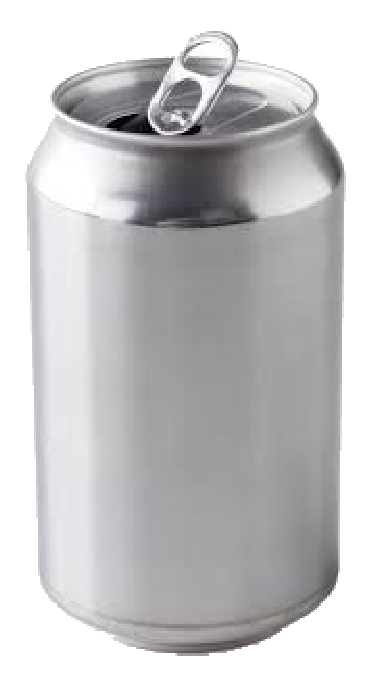
\includegraphics[width=2.5cm]{Grandeurs_mesures/Images/M14_ex_canette}
   \end{center}
   \begin{enumerate}
      \item Déterminer, au dixième de gramme près, la masse d’aluminium nécessaire pour fabriquer une cannette classique.
      \item Il faut \ukg{9} d’aluminium pour fabriquer un certain type de vélo. Estimer le nombre de cannettes classiques nécessaires pour obtenir l’aluminium pour fabriquer un tel vélo.
   \end{enumerate}
\end{exercice}

\begin{corrige}
\ \\ [-5mm]
   \begin{enumerate}
      \item
         \begin{itemize}
            \item Calcul du volume d'aluminium nécessaire pour fabriquer le corps de la canette : \\
               $130\,\mu\um{} =130\times10^{-6}\um{} =130\times10^{-4}\,\ucm{} =\ucm{0,013}$. \\
               $\mathcal{V} =\text{surface}\times\text{épaisseur} =\ucmq{268,42}\times\ucm{0,013} \approx\ucmc{3,49}$. \\
            \item Calcul de la masse d'aluminium nécéssaire pour fabrique le corps de la canette : \\ [1mm]
               la masse volumique de l'aluminium vaut $\mu =\dfrac{\ukg{2700}}{\umc{1}} =\dfrac{\ug{2700000}}{\ucmc{1000000}} =2,7\text{ g/cm}^3$. \\ [1mm]
               Un volume de \ucmc{3,49} d'aluminium a une masse $m$ en gramme égale à $3,49\times2,7 \approx9,423$.
            \item Calcul de la masse totale d'aluminium nécéssaire pour la canette entière : \\
               $M =$ masse du corps + masse de l'anneau + masse de soudure \\
               $M \approx\ug{9,4}+\ug{1,4}+\ug{1,9} \approx\ug{12,7}$. \\
               {\blue Il faut environ \ug{12,7} d'aluminium pour fabriquer une canette classique}.
         \end{itemize}
      \item Pour un vélo de \ukg{9}, soit \ug{9000}, on effectue le calcul suivant : \\
         $\ug{9000}\div\ug{12,7} \approx 708,66$. \\
         {\blue Il faudrait environ 709 canettes classiques pour fabriquer ce type de vélo}.
   \end{enumerate}
\end{corrige}

\bigskip


\begin{exercice}[CRPE 2018 G1-G3] %%%8
   Pour chacune des affirmations suivantes indiquer si elle est vraie ou fausse, en justifiant la réponse. \\
   Une réponse exacte mais non justifiée ne rapporte aucun point. Une réponse fausse n'enlève pas de point.
   \begin{enumerate}
      \item On considère un cube dont la surface totale extérieure mesure \ucmq{576}. \\
         {\bf Affirmation 1:} Son volume est inférieur à 1 litre.
      \item {\bf Affirmation 2 :} Les dimensions de mon échantillon de parfum sont cinq fois plus petites que celles de mon flacon habituel. Il y a donc 25 fois moins de parfum dans l’échantillon que dans le flacon habituel.
   \end{enumerate}
\end{exercice}

\begin{corrige}
\ \\ [-5mm]
   \begin{enumerate}
      \item Un cube possède six faces isométriques, donc si la surface totale extérieure mesure \ucmq{576}, une face a pour aire \ucmq{96} ($576\div6 =96$). \\
         Le côté du carré, et donc du cube mesure $\sqrt{96}$ cm et le volume a pour mesure : \\
         $(\sqrt{96}\,\ucm{})^3 \approx \ucmc{941} \approx \udmc{0,941} \	\approx \ul{0,941}$ ce qui est inférieur à \ul{1}. \\
         {\blue L'affirmation est vraie} \\
      \item La réduction des dimensions d'un objet par 5 diminue les aires par $5^2 =25$ et les volumes et capacités par $5^3 =125$. \\
         {\blue L'affirmation est fausse.}
   \end{enumerate}
\end{corrige}

\bigskip


\begin{exercice}[CRPE blanc 2019 Réunion] %%%9
   La nuit dernière, un crime s’est déroulé au {\it Gîte des hauts}, gîte spécialisé dans les tentes atypiques : monsieur Mathrice a été assassiné dans sa tente puis déplacé à l'accueil. \\ [-8mm]
   \begin{center}
      {\hautab{1.5}
      \begin{tabular}{|C{8}|C{8}|}
         \hline
         \bf Tente 1 & \bf Tente 2 \\
         \begin{pspicture}(-1,-0.3)(4.5,3.5)
            \psset{unit=0.8}
            \psline(0,0)(3,0)(4,1)
            \psline[linestyle=dashed](4,1)(1,1)(0,0)
            \psline(0,0)(2,4)(4,1)
            \psline(3,0)(2,4)
            \psline[linestyle=dashed](1,1)(2,4)
            \psline[linestyle=dotted](0,0)(4,1)
            \psline[linestyle=dotted](2,4)(2,0.5)
            \psline[linestyle=dotted](3,0)(1,1)
            \pcline[offset=10pt]{<->}(2,4)(4,1) \mput*{$\ell$}
            \pcline[offset=-10pt]{<->}(0,0)(3,0) \mput*{$c$}
            \rput(2,0.25){\footnotesize $O$}
            \rput(2.2,1.7){$h$}
         \end{pspicture}
         &
         \begin{pspicture}(-1,-0.3)(4.5,3.5)
            \psset{unit=1.1}
            \pspolygon(0,0)(2,0)(3,1)(3,3)(1,3)(0,2)
            \psline(0,2)(2,2)(2,0)
            \psline(2,2)(3,3)
            \psline[linestyle=dashed](0,0)(1,1)(3,1)
            \psline[linestyle=dashed](1,1)(1,3)
            \pcline[offset=-10pt]{<->}(0,0)(2,0) \mput*{$c$}
         \end{pspicture}
         \\
         Base carrée de centre $O$, la hauteur $h$ est perpendiculaire à la base. $c =\um{3,7}$ et $\ell =\um{3,2}$. 
         &
         Toutes les faces sont des carrés, deux faces consécutives sont orthogonales. $c =\um{1,9}$. \\
         \hline
         \bf Tente 3 & \bf Tente 4 \\
         \begin{pspicture}(-2,-2)(4,2)
            \psset{unit=1.1}
            \pspolygon(1;30)(1;90)(1;150)(1;210)(1;270)(1;330)
            \psframe(0.87,-0.5)(1.62,0.5)
            \rput(0,0){\small$\mathcal{A} =6\sqrt3\umq{}$}
            \rput{60}(0,0){\psframe(0.87,-0.5)(1.62,0.5)}
            \rput{120}(0,0){\psframe(0.87,-0.5)(1.62,0.5)}
            \rput{180}(0,0){\psframe(0.87,-0.5)(1.62,0.5)}
            \rput{240}(0,0){\psframe(0.87,-0.5)(1.62,0.5)}
            \rput{300}(0,0){\psframe(0.87,-0.5)(1.62,0.5)}
            \rput(2.49,0){\pspolygon(1;30)(1;90)(1;150)(1;210)(1;270)(1;330)}
            \pcline[offset=-6pt]{<->}(1;150)(1;-150) \mput*{$b$}
            \pcline[offset=-10pt]{<->}(0.87;0)(1.62;0) \mput*{$a$}
         \end{pspicture}
         &
         \begin{pspicture}(-1,0)(5,4)
            \psset{unit=0.6}
            \psline(5,1.1)(3,6)(1,1.1)
            \psellipticarc(3,1)(2,1){180}{0}
            \psellipticarc[linestyle=dashed](3,1)(2,1){0}{180}
            \psline[linestyle=dotted](3,1)(3,6)
            \rput(2.7,3){$h$}
            \pcline{<->}(3,1)(5,1) \mput*{$r$}
            \psarc(3,6){1.5}{-90}{-67}
            \psarc(3,6){1.65}{-90}{-67}
            \rput(3.4,3.8){$\alpha$}
            \rput(3,0.6){\footnotesize $O$}
         \end{pspicture}
         \\
         Patron d'un solide, les hexagones sont réguliers, les rectangles sont identiques. $a =\um{1,8}$ et $b =\um{4}$. 
         &
         Base circulaire de centre $O$, la hauteur $h$ est perpendiculaire à la base. $r =\um{1,5}$ et $\alpha =35\degres$. \\
         \hline
      \end{tabular}}
   \end{center}
   \begin{enumerate}
      \item Nommer les quatre solides formant les quatre tentes.
      \item
         \begin{enumerate}
            \item Donner la hauteur des tentes 2 et 3.
            \item Déterminer la hauteur de la tente 4 (arrondir au cm).
            \item Déterminer la hauteur de la tente 1 (arrondir au cm).
         \end{enumerate}
      \item Donner le volume de chaque tente au mètre cube près.
      \item Monsieur Mathrice mesurait 1 m 92, il avait donc demandé une tente suffisamment grande pour qu'il puisse tenir debout en son centre. En déduire le lieu où il a été assassiné.
   \end{enumerate}
\end{exercice}

\begin{corrige}
\ \\ [-5mm]
   \begin{enumerate}
      \item La tente 1 est une {\blue pyramide} à base carrée, la tente 2 est un {\blue cube}, la tente 3 est un {\blue prisme} à base hexagonale et la tente 4 est un {\blue cône.}
      \item
         \begin{enumerate}
            \item La tente 2 est un cube, sa hauteur est {\blue $c =\um{1,9}$} et la tente 3 est un prisme de hauteur {\blue $a =\um{1,8}$}.
            \item On appelle $S$ le sommet du cône et $A$ un point du cercle de base, dans le triangle $SOA$ rectangle en $O$ (la hauteur $h$ est perpendiculaire à la base), on a : $\tan(\widehat{OSA}) =\dfrac{OA}{h}$ d'où $h =\dfrac{r}{\tan(\alpha)} =\dfrac{\um{1,5}}{\tan{\udeg{35}}} \approx\um{2,14}$. \\ [1mm]
               La tente 4 a pour {\blue hauteur \um{2,14}} environ.
            \item On appelle $S$ le sommet de la pyramide et $A$ un sommet du carré de base, la diagonale du carré a pour mesure $c\sqrt{2}\,\um{}$ et donc sa demi-diagonale mesure $c\sqrt{2}/2\,\um{}$. Dans le triangle $SOA$ rectangle en $O$ (la hauteur est perpendiculaire à la base), on a d'après le théorème de Pythagore, avec des mesure en \um{} : \\
               $SA^2 =SO^2+OA^2 \iff \ell^2 =h^2+\left(\dfrac{c\sqrt{2}}{2}\right)^2 \iff h^2 =3,2^2-(1,85\sqrt2)^2 \iff h^2 =3,395$. \\ [1mm]
               La tente 1 a pour {\blue hauteur \um{1,84}} environ.
         \end{enumerate}
      \setcounter{enumi}{2}
      \item
         \begin{itemize}
            \item $\mathcal{V}_{\text{tente 1}} =\dfrac13\times\mathcal{A}_{\text{base}}\times h=(\um{3,7})^2\times\um{1,84} \approx\umc{8,40} \approx{\blue\umc{8}}$. \smallskip
            \item $\mathcal{V}_{\text{tente 2}} =c^3=(\um{1,9})^3 \approx\umc{6,86} \approx{\blue \umc{7}}$.
            \item $\mathcal{V}_{\text{tente 3}} =\mathcal{A}_{\text{base}}\times a=6\sqrt3\,\umq{}\times\um{1,8} \approx\umc{18,71} \approx{\blue \umc{19}}$. \smallskip
            \item $\mathcal{V}_{\text{tente 4}} =\dfrac13\times\mathcal{A}_{\text{base}}\times h=\pi\times(\um{1,5})^2\times\um{2,14} \approx\umc{5,04} \approx{\blue \umc{5}}$. \smallskip
         \end{itemize}
      \item M. Mathrice était hébergé dans la {\blue tente 4}, la seule ayant une hauteur supérieure à sa taille.
   \end{enumerate}
\end{corrige}


\begin{exercice}[CRPE 2009 G4] %%%%%%%%%%%%%%%%%%%%
  \begin{minipage}{14cm}
     On a représenté ci-contre un tube creux en aluminium en perspective. \\
     Son diamètre intérieur est 8 cm, son diamètre extérieur est 12 cm. \\
     L'aluminium a une masse volumique de 2,7 g/cm$^3$. On veut transporter un certain nombre de ces tubes dans un camion dont la charge utile ne peut dépasser 14 tonnes. \\
     En supposant que le volume du camion est suffisant, combien peut-on transporter de tubes au maximum ? \textit{On utilisera 3,14 comme valeur approchée de $\pi$.}
  \end{minipage}
  \qquad 
  \begin{minipage}{3cm}
     {\psset{yunit=0.8}
     \begin{pspicture}(0,-0.5)(2.5,3.5)
        \psellipse(0.25,0)(0.25,0.15)
        \psframe[fillstyle=solid,fillcolor=white,linecolor=white](0,0)(0.5,5)
        \psline(0,0)(0,5)
        \psline(0.5,0)(0.5,5)
        \psellipse(0.25,5)(0.25,0.15)
        \psellipse(0.25,5)(0.15,0.05)
        \psline{|-|}(1,0)(1,5)
        \rput(1.75,2.5){\ucm{75}}
     \end{pspicture}}
  \end{minipage}  
\end{exercice}

\begin{corrige} 
\begin{itemize}
   \item Volume d'un tube creux : il correspond au volume d'un tube plein de rayon 6 cm, auquel on enlève le volume d'un tube plein de rayon 4 cm. \\
   -- Volume du cylindre de 6 cm de rayon en cm$^3$ : $\mathcal{V}_1= 3,14\times6^2\times75 =8\,478$. \\
   -- Volume du cylindre de 4 cm de rayon  en cm$^3$ : $\mathcal{V}_2= 3,14\times4^2\times75 =3\,768$. \\
   Donc, le volume du tube creux est de $\ucmc{8478}-\ucmc{3768} = \ucmc{4710}$.
   \item Masse d'un tube creux : la masse volumique du tube est de 2,7g\,\slash cm$^3$. \\
   Or, $2,7\times4\,710 =12\,717$, donc, la masse du tube creux est de 12 717 g = 12,717 kg.
   \item Nombre de tubes à transporter : la charge utile du camion est de 14 tonnes, soit 14 000 kg. \\ [1mm]
   Or, $\dfrac{14\,000}{12,717} \approx1\,100,89$ donc, {\blue le camion peut transporter au maximum 1 100 tubes creux en aluminium.}
\end{itemize}
\end{corrige}



%\begin{exercice*}[CRPE 2005 Dijon] %%%%%%%%%%%%%
%   Depuis ce matin, un magasinier range sans interruption des caisses dans un entrepôt. \\
%   Il a calculé que, s'il range 50 caisses à l'heure, il aura fini à 11h30. \\
%   Si par contre, il en range 60 à l'heure, il aura fini à 11 h15. \\
%   A quelle heure a-t-il commencé son travail ? Justifier la réponse.
%\end{exercice*}
%
%\begin{corrige}
%Soit $n$ le nombre de caisses à transporter, $t_1$, le temps mis (en minutes) pour ranger les caisses à une \og vitesse \fg{} de 50 caisses par heure, c'est à dire $\dfrac56$ de caisse par minute et $t_2$ le temps mis à une \og vitesse \fg{} de 60 caisses par heure, c'est-à-dire une caisse par minute.
%\begin{center}
%\begin{pspicture}(0,-1)(6,2)
%   \pcline{|->}(0,0)(5,0)
%   \lput*{:U}{$t_2$}
%   \rput(5,-0.4){11h15}
%   \pcline{|->}(0,1)(6,1)
%   \lput*{:U}{$t_1$}
%   \rput(6,0.6){11h30}
%   \psline[linestyle=dashed](0,-0.5)(0,1.5)
%\end{pspicture}
%\end{center}
%   On a : $t_1-t_2 =15 \quad ; \quad \dfrac56 =\dfrac{n}{t_1} \quad \text{ et } \quad 1 =\dfrac{n}{t_2}$, \quad ou encore $n =\dfrac56t_1$ et $n =t_2$. \\ [1mm]
%   On obtient le système : $\syst{t_1-t_2 &=&15}{\dfrac56t_1 &=&t_2} \iff \syst{t_1 &=&t_2+15}{5t_1 &=&6t_2} \iff \syst{t_1 &=&t_2+15}{5(t_2+15) &=&6t_2}$ \\ [1mm]
%   \hspace*{2.5cm} $\iff \syst{t_1 &=&t_2+15}{5t_2+75 &=&6t_2} \iff \syst{t_1 &=&t_2+15}{75 &=&6t_2-5t_2} \iff \syst{t_1 &=&75+15=90}{t_2 &=&75}$ \\ [3mm]
%  On a, par exemple, $t_2 =\umin{75}$, soit 1 h 15 min et 11 h 15 min - 1 h 15 min = 10 h 00. \\
%  Donc, {\blue le magasinier a commencé son travail à 10h00.} \\
%\end{corrige}




